\phantomsection

\chapter{Pre-Exploitation}
\markboth{Pre-Exploitation}{}

\section{Target Scoping} { \setstretch{1.3}}
Il processo di \emph{Penetration Testing}, come evidenziato nella fase introduttiva, ha uno scopo puramente didattico, per cui non è prevista una fase di accordo tra le parti coinvolte in quanto l'asset da analizzare è una macchina virtuale vulnerabile \emph{by design}. Non vi è, infatti, un cliente dal quale raccogliere requisiti e con il quale definire obiettivi di business e modelli dei costi. Il processo verrà svolto senza particolari vincoli formali relativi all'asset.

\section{Information Gathering} { \setstretch{1.3}}
La caratterizzazione dell'asset da analizzare può generalmente avvenire mediante molteplici \emph{tool} e coinvolgere diversi aspetti dell'asset stesso. Dal momento che si sta trattando una macchina virtuale vulnerabile \emph{by-design} contestualizzata in un'attività progettuale avente uno scopo didattico non risulta utile ricorrere a particolari tecniche \emph{OSINT (Open Source INTelligence)}, né a tecniche volte all'ottenimento di informazioni di routing e record DNS. Sono state, tuttavia, consultate le informazioni di base dell'asset disponibili sulla piattaforma \emph{VulnHub} che mette a disposizione la macchina virtuale. Le informazioni fornite sono le seguenti:
\begin{itemize}
    \item \textbf{Nome della macchina}: \emph{Momentum: 1};
    \item \textbf{Sistema Operativo}: \emph{Linux};
    \item \textbf{DHCP Server}: abilitato;
    \item \textbf{Indirizzo \emph{IP}}: assegnato in automatico.
\end{itemize}
Non risultano, dunque, note le informazioni relative all'indirizzo \emph{IP} della macchina né le credenziali di accesso alla stessa. 
\section{Target Discovery} { \setstretch{1.3}}
L'individuazione della macchina \emph{Momentum: 1} all'interno della rete è stata effettuata, in accordo con quanto descritto nel capitolo introduttivo, utilizzando una macchina virtuale con \emph{Kali Linux} connessa alla medesima rete. 
\subsection{Informazioni preliminari}
Prima di procedere alla trattazione delle metodologie di individuazione della macchina target è necessario considerare alcuni aspetti dell'architettura di rete virtuale nell'ambito della quale è stata svolta l'attività di \emph{Penetration Testing}. La gestione del \emph{NAT} e del \emph{DHCP} da parte di \emph{VirtualBox} fa sì che risultino connessi alla rete degli host aventi \emph{IP} \emph{10.0.2.1}, \emph{10.0.2.2} e \emph{10.0.2.3}. Alla rete risulterà altresì connessa la macchina virtuale con \emph{Kali Linux} della quale è stato rilevato l'indirizzo \emph{IP} (\emph{10.0.2.15}) mediante il comando \emph{ifconfig} il cui output è illustrato nella figura \ref{fig:ifconfig}. 
\begin{figure}[h]
    \centering
    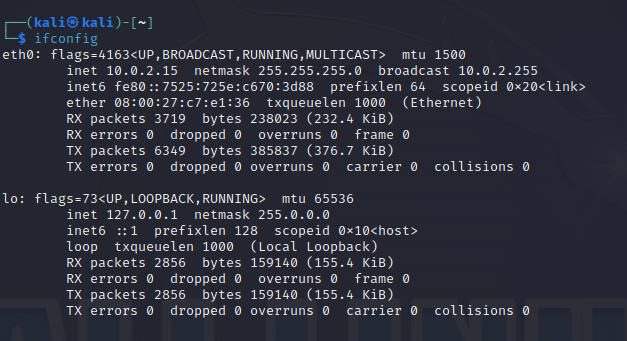
\includegraphics[scale=0.8]{capitoli/images/ifconfig.png}
    \caption{Output del comando \emph{ifconfig}}
    \label{fig:ifconfig}
\end{figure}
\subsection{Scansione con \emph{nmap}}
Come evidenziato in precedenza, l'indirizzo \emph{IP} di \emph{Momentum: 1} non è noto in quanto viene assegnato mediante il servizio di \emph{DHCP} di \emph{VirtualBox}. Per tale ragione è stata eseguita una scansione volta alla rilevazione della macchina target sulla rete \emph{10.0.2.0/24} mediante il comando:
\begin{lstlisting}[language=bash]
    $ nmap -sP 10.0.2.0/24
\end{lstlisting}
Questo comando effettua un \emph{ping scan} di tutti gli host della rete specificata in input \cite{nmap}, nell'ambito della quale vengono rilevati 3 host attivi, come mostrato nella figura \ref{fig:nmap}. Dal momento che, come specificato in precedenza, l'indirizzo \emph{10.0.2.1} fa riferimento ad un host di \emph{VirtualBox} e l'indirizzo \emph{10.0.2.15} è relativo alla macchina virtuale con \emph{Kali}, risulta immediato stabilire che l'indirizzo \emph{IP} di \emph{Momentum: 1} è \emph{10.0.2.4}.
\begin{figure}[h]
    \centering
    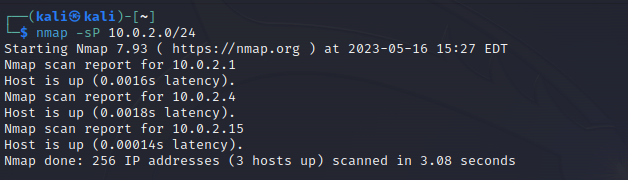
\includegraphics[scale=0.75]{capitoli/images/nmap.png}
    \caption{Output del comando \emph{nmap (ping scan)}}
    \label{fig:nmap}
\end{figure}
\subsection{Determinazione \emph{MAC Address} con \emph{arping}}
A partire dall'indirizzo \emph{IP} di \emph{Momentum: 1}, risulta possibile arricchire la conoscenza della macchina target individuandone il \emph{MAC Address}. Ciò è possibile mediante il comando:
\begin{lstlisting}[language=bash]
    $ sudo arping 10.0.2.4 -c 1
\end{lstlisting}
Tale comando invia un'\emph{ARP Request} al dispositivo indicato in input \cite{arping}. Mediante l'output, illustrato nella figura \ref{fig:arping}, si stabilisce che il \emph{MAC Address} di \emph{Momentum: 1} è \emph{08:00:27:0f:15:fd}.
\begin{figure}[h]
    \centering
    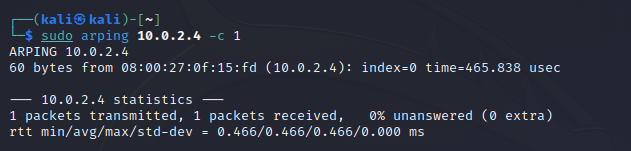
\includegraphics[scale=0.75]{capitoli/images/arping.png}
    \caption{Output del comando \emph{arping}}
    \label{fig:arping}
\end{figure}
\subsection{Scansione con \emph{arp-scan}}
Durante il processo di \emph{Penetration Testing} è stato utilizzato un approccio volto all'ottenimento delle medesime informazioni mediante molteplici tool al fine di confrontarne i risultati per massimizzare il quantitativo di informazioni ottenute nell'ambito di una determinata fase. A tale scopo ci si è serviti del tool \emph{arpscan} per effettuare una scansione sulla rete \emph{10.0.2.0/24} mediante il comando:
\begin{lstlisting}[language=bash]
    $ sudo arp-scan 10.0.2.0/24
\end{lstlisting}
\begin{figure}
    \centering
    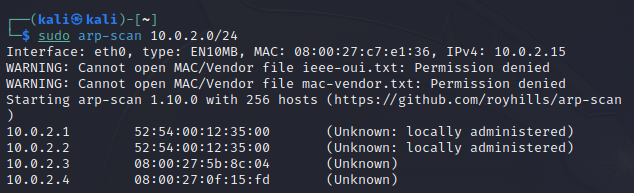
\includegraphics[scale=0.75]{capitoli/images/arpscan.png}
    \caption{Output del comando \emph{arp-scan}}
    \label{fig:arpscan}
\end{figure}
L'output del comando, illustrato nella figura \ref{fig:arpscan}, mostra che la scansione ha rilevato 4 host, per ciascuno dei quali ha fornito il relativo indirizzo \emph{IP} ed il relativo \emph{MAC Address}. La precedente scansione (effettuata con il tool \emph{nmap}) non ha rilevato gli host \emph{192.168.1.2} e \emph{192.168.1.3}, tuttavia, come evidenziato in precedenza, questi host sono gestiti da \emph{VirtualBox} per cui non hanno rilevanza nel processo di \emph{Penetration Testing} effettuato. L'host avente indirizzo \emph{IP} \emph{10.0.2.4} e \emph{MAC Address 08:00:27:0f:15:fd} è relativo alla macchina target.
\subsection{OS Fingerprinting attivo con \emph{nmap}}
Al fine di arricchire la conoscenza relativa alla macchina target è stata effettuata un'operazione di \emph{OS detection} mediante il comando:
\begin{lstlisting}[language=bash]
    $ sudo nmap -O 10.0.2.4
\end{lstlisting}
\begin{figure}
    \centering
    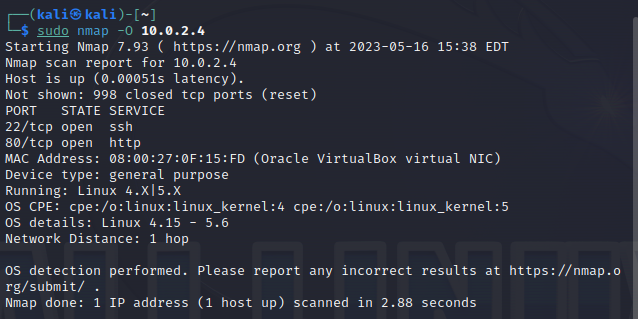
\includegraphics[scale=0.75]{capitoli/images/fingerprinting.png}
    \caption{Output del comando \emph{nmap (SO Fingerprinting)}}
    \label{fig:fingerprinting}
\end{figure}
L'output ottenuto (figura \ref{fig:fingerprinting}) fornisce diverse informazioni relative al sistema operativo in esecuzione sulla macchina target. È possibile stabilire che si tratta di un sistema \emph{Linux} presumibilmente ad una versione \emph{4.15} o \emph{5.6} (quando \emph{nmap} non riesce a stabilirlo con precisione mostra tutte i possibili match \cite{nmap-manual}); il tool fornisce, infine, la \emph{CPE} \footnote{\emph{CPE (Common Platform Enumeration)} è un sistema di naming strutturato per sistemi operativi, software e packages \cite{cpe}} di riferimento (\emph{cpe:/o:linux:linux\_kernel:4 cpe:/o:linux\_kernel:5}). Sono, altresì, presenti informazioni relative alle porte aperte ed ai servizi attivi sulla macchina target, che nell'ambito della fase di \emph{Target Discovery}, sono state sfruttate unicamente per effettuare OS Fingerprinting passivo; sulla macchina target risultano aperte la porta 80 (servizio \emph{HTTP}) e la porta 22 (servizio \emph{SSH}).
\subsection{OS Fingerprinting passivo con \emph{p0f}}
La fase di OS Fingerprinting attivo non ha portato all'individuazione dell'esatta versione del sistema operativo in esecuzione sulla macchina target: è stata, dunque, svolta una fase di OS Fingerprinting passivo, finalizzata all'ottenimento di ulteriori informazioni in merito, utilizzando il tool \emph{p0f}. La tecnica di fingerprinting passivo adottata consiste nel porsi in ascolto su una specifica interfaccia di rete ed ispezionare i pacchetti \emph{TCP/IP} intercettati al fine di individuare le informazioni desiderate. Tale operazione è stata svolta mediante il comando:
\begin{lstlisting}[language=bash] 
    $ sudo p0f -i eth0 
\end{lstlisting}
Il passo successivo consiste nel fare in modo che la macchina target invii pacchetti sull'interfaccia di rete \emph{eth0}; a tale scopo sono state effettuate delle richieste ai servizi esposti dalla macchina, ossia \emph{HTTP} e \emph{SSH}, mediante i comandi:
\begin{lstlisting}[language=bash] 
    $ curl -X GET http://10.0.2.4/
    $ ssh user@10.0.2.4
\end{lstlisting}
A tali richieste corrispondono delle risposte, intercettate dal tool \emph{p0f} e dalle quali sono state ottenute le informazioni riportate nelle figure \ref{fig:p0f_http} e \ref{fig:p0f_ssh}.
\begin{figure}[h]
    \centering
    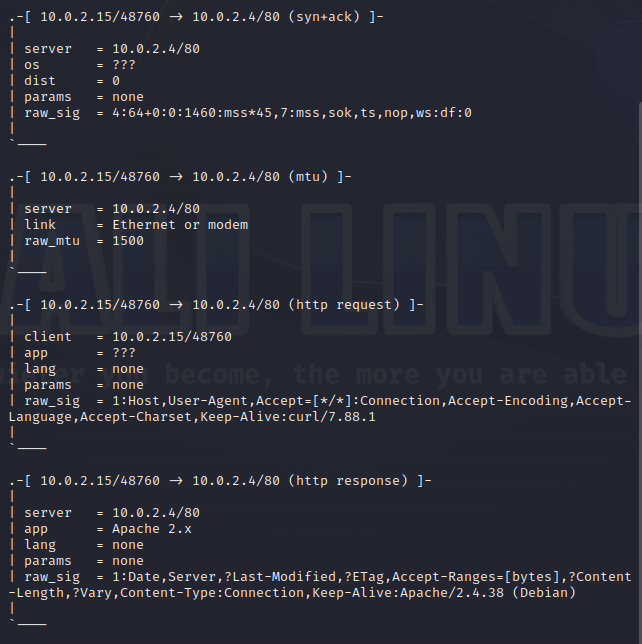
\includegraphics[scale=0.7]{capitoli/images/p0f_http.png}
    \caption{Output del comando \emph{p0f} (risposta \emph{HTTP})}
    \label{fig:p0f_http}
\end{figure}
\begin{figure}[h]
    \centering
    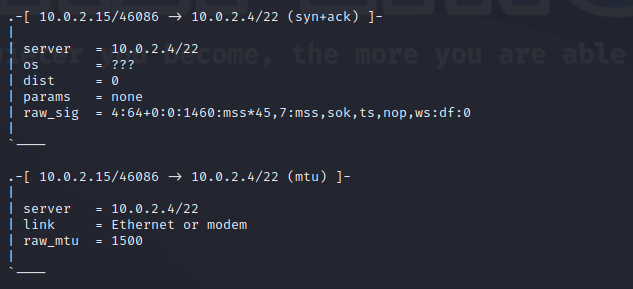
\includegraphics[scale=0.7]{capitoli/images/p0f_ssh.png}
    \caption{Output del comando \emph{p0f} (risposta \emph{SSH})}
    \label{fig:p0f_ssh}
\end{figure}
Dalle sezioni relative alla macchina target (che riportano il parametro \emph{server} uguale a \emph{10.0.2.4/80} o a \emph{10.0.2.4/22}) si evince che il tool \emph{p0f} non è riuscito a stabilire la versione del sistema operativo in esecuzione in quanto al parametro \emph{os} è associata la stringa \emph{`???'}. L'operazione di OS Fingerprinting passivo non ha, dunque, condotto ai risultati sperati in quanto non è stato possibile arricchire ulteriormente la conoscenza relativa alla versione del sistema operativo in esecuzione.  
\section{Target Enumeration} { \setstretch{1.3}}
Nel corso delle precedenti fasi sono state svolte diverse scansioni volte al rilevamento della macchina target sulla rete virtuale. Tali scansioni hanno portato alla scoperta di alcuni servizi in esecuzione sulla macchina target, che nell'ambito della fase di \emph{Target Enumeration} sono stati ulteriormente caratterizzati. 
\subsection{\emph{TCP} port scanning con \emph{nmap}}
L'utilizzo del tool \emph{nmap} risulta utile anche durante la fase di \emph{TCP port scanning} in quanto, mediante le opzioni messe a disposizione, è possibile eseguire diversi tipologie di scansioni volte al rilevamento delle porte \emph{TCP} aperte. Consultando la pagina del manuale di \emph{Linux} relativa ad \emph{nmap} \cite{nmap} è stato scoperto che l'opzione \emph{-A} consente di effettuare un'\emph{aggressive scan} che consiste in operazioni di \emph{OS detection, version scanning, script scanning} e \emph{traceroute}. Tale tipo di scansione risulta essere particolarmente efficace in quanto in grado di rilevare un maggior numero di informazioni rispetto alle altre tipologie di scansioni disponibili. È stato, dunque, eseguito il seguente comando: 
\begin{lstlisting}[language=bash] 
    $ nmap -A 10.0.2.4 -p- -oX aggressive_scan.xml
\end{lstlisting}
L'opzione \emph{-p-} indica che il range di porte da scansionare va da \emph{1} a \emph{65535}, mentre l'opzione \emph{-oX} serve per salvare l'output del tool in formato \emph{XML} sul file \emph{aggressive\_scan}. Al fine di agevolarne la consultazione, il file è stato opportunamente convertito in \emph{HTML} mediante il comando:
\begin{lstlisting}[language=bash]
    $ xsltproc aggressive_scan.xml -o aggressive_scan.html
\end{lstlisting}
\begin{figure}[h]
    \centering
    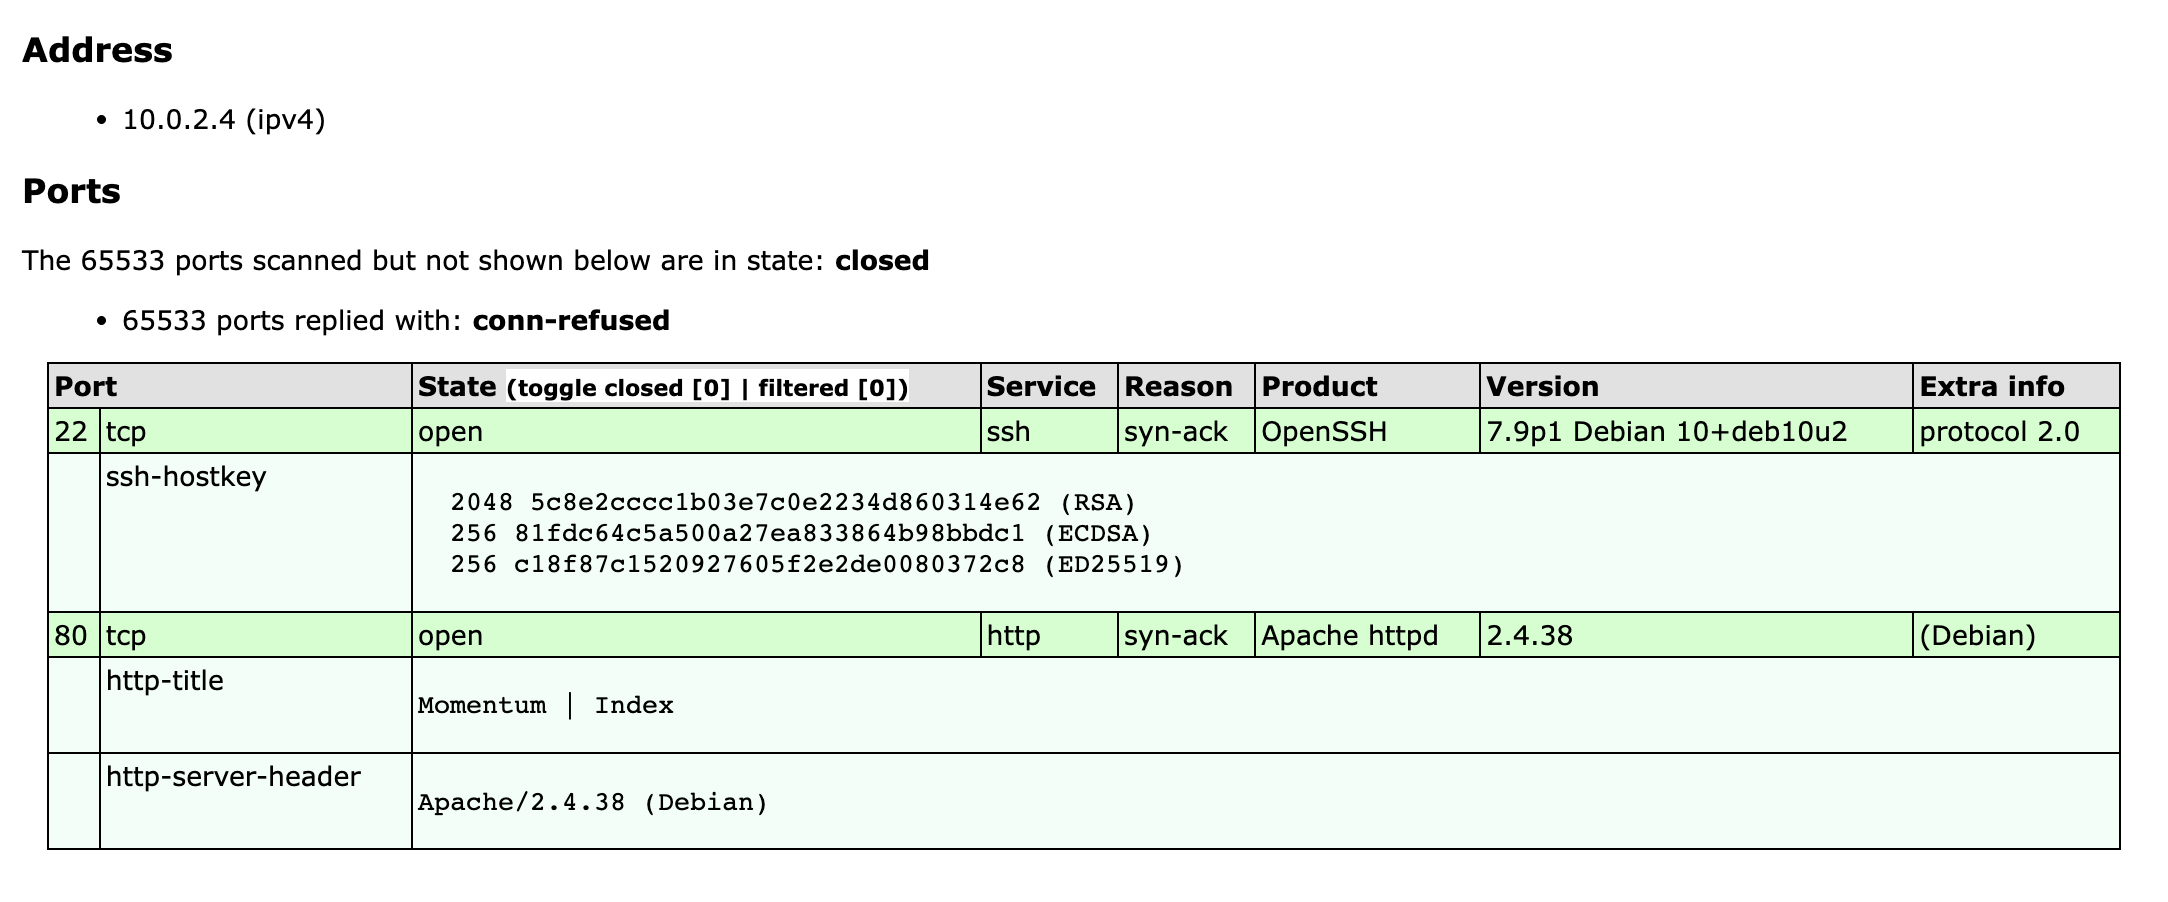
\includegraphics[scale=0.45]{capitoli/images/aggressive_scan.png}
    \caption{Output del comando \emph{nmap} (aggressive scan)}
    \label{fig:aggressive_scan}
\end{figure}
Il risultato dell'aggressive scan (illustrato nella figura \ref{fig:aggressive_scan}) è reperibile al link: e fornisce svariate informazioni relative allo stato delle porte \emph{TCP} della macchina target. Come già rilevato dalla scansione eseguita nell'ambito della fase di \emph{SO Fingerprinting}, le porte 22 e 80 risultano aperte e sono utilizzate rispettivamente da un server \emph{SSH} e da un server \emph{HTTP}. Sono, altresì, riportati i valori delle chiavi pubbliche impiegate dagli algoritmi di autenticazione di \emph{SSH} (\emph{RSA, ECDSA, ED25519}), il nome della pagina di default del server \emph{HTTP} (\emph{Momentum | Index}) e le informazioni sulla versione del server \emph{HTTP} (\emph{Apache/2.4.38 (Debian)}). Un'ulteriore informazione di estrema importanza riguarda lo stato delle restanti \emph{65533} porte che, avendo risposto con un messaggio di \emph{conn-refused}, risultano senza dubbio chiuse; non sono, dunque, necessarie ulteriori scansioni per le porte \emph{TCP}. 
\subsection{\emph{UDP} port scanning con \emph{unicornscan}}
Dal momento che il tool \emph{nmap} risulta inefficiente nell'ambito delle scansioni \emph{UDP}, è stato utilizzato il tool \emph{unicornscan}:
\begin{lstlisting}[language=bash]
    $ sudo unicornscan -m U -Iv 10.0.2.4:1-65535
\end{lstlisting}
L'opzione \emph{-m U} indica la tipologia di scansione da eseguire (\emph{UDP}), mentre l'opzione \emph{-Iv} specifica che l'output deve essere stampato a schermo in tempo reale e che deve essere di tipo \emph{verbose}. È stato, infine, specificato l'indirizzo \emph{IP} dell'host da scansionare con il relativo range di porte (da 1 a 65535).  
\begin{figure}[h]
    \centering
    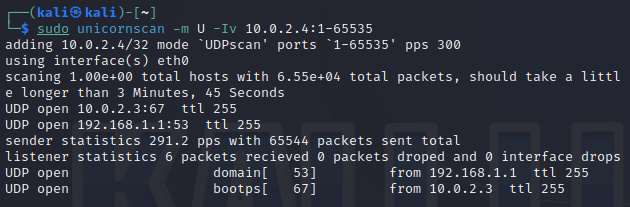
\includegraphics[scale=0.7]{capitoli/images/udp.png}
    \caption{Output del comando \emph{unicornscan}}
    \label{fig:unicornscan}
\end{figure}
I risultati, illustrati nella figura \ref{fig:unicornscan}, mostrano che le porte \emph{UDP} rilevate non sono relative alla macchina target, bensì al router e ad un host virtuale di \emph{VirtualBox} e fanno riferimemento rispettivamente al servizio \emph{Domain Name System (DNS)} e al servizio \emph{Bootstrap Protocol Server (BPS)} (l'elenco delle porte ben note è regolato dallo standard \emph{RFC 1340} \cite{rfc1340}). Tali porte sono state rilevate in quanto \emph{unicornscan} segnala come aperte le porte relative agli host da cui riceve dei pacchetti sulla rete \cite{unicornscan}. Si può, dunque, concludere che non vi sono porte \emph{UDP} aperte sulla macchina target. 
\section{Vulnerability Mapping}
Individuati i servizi erogati dalla macchina target, risulta opportuno svolgere una fase volta all'identificazione delle vulnerabilità della stessa. Nell'ambito di tale analisi ci si avvarrà sia di strumenti preinstallati in \emph{Kali Linux} che di strumenti appositamente installati e configurati. L'utilizzo di molteplici tool risulta cruciale in tale fase in quanto le modalità di rilevazione delle vulnerabilità si basano su euristiche estremamente variabili. Le successive sezioni sono dedicate alla trattazione dei tool impiegati e delle relative vulnerabilità rilevate.
\subsection{OpenVAS}
\emph{OpenVAS} (Open Vulnerability Assesment System) è un security scanner open source facilmente installabile su \emph{Kali Linux}. Mediante la sua interfaccia \emph{Web-based} sono stati configurati i parametri necessari allo svolgimento della scansione sulla macchina target; in particolare:
\begin{itemize}
    \item Sono state scansionate tutte le 65535 porte;
    \item È stato utilizzato un \emph{Minimum Quality of Detection} del 70\% in modo da avere un soddisfacente compromesso tra rilevamento delle vulnerabilità e rischio di incorrere in falsi positivi;
    \item È stato utilizzato lo scanner di default di \emph{OpenVAS}, che fa uso delle informazioni fornite dai servizi di feed \emph{NVT, SCAP, CERT} e \emph{GVMD DATA};
    \item La configurazione impiegata per le scansioni è \emph{`Full and fast'}.
\end{itemize}
La scansione ha richiesto circa 14 minuti generando un report (\emph{`openvas-report.pdf'}) reperibile nella directory \emph{tools-output} (o al seguente link: ). Sono state rilevate due vulnerabilità aventi una severity bassa:
\begin{itemize}
    \item \textbf{[Severity: 2.6]} \textbf{TCP Timestamps Information Disclosure}: la macchina target implementa la rilevazione dei timestamp via \emph{TCP} dando la possibilità di computarne l'uptime;
    \item \textbf{[Severity: 2.1]} \textbf{ICMP Timestamp Reply Information Disclosure} (\emph{CVE-1999-0524}): la macchina target ha risposto ad una richiesta \emph{ICMP} di timestamp. Tale informazione potrebbe essere sfruttata per violare generatori di numeri casuali \emph{time-based} deboli presenti in servizi eventualmente installati sulla macchina target.
\end{itemize}
La scansione effettuata con \emph{OpenVAS} non ha rilevato vulnerabilità gravi, bensì comportamenti dannosi sfruttabili da attaccanti sotto determinate condizioni.
\subsection{Nessus}
\emph{Nessus} è un software proprietario che mette a disposizione diversi piani di utilizzo, tra cui il piano \emph{Esssentials} gratuito, provvisto di funzionalità limitate ed utilizzato nell'ambito del presente processo di \emph{Penetration Testing}. Questo tool consente di effettuare numerose tipologie di scansioni, alcune delle quali sono disponibili con il piano \emph{Essentials}. In totale sono state effettuate due differenti scansioni, ciascuna configurata con opportuni parametri:
\begin{itemize}
    \item 
\end{itemize}
\subsection{DIRB}
\subsection{Nikto2}
\subsection{OWASP ZAP}
\subsection{Paros Proxy}
\subsection{WhatWeb}
\subsection{WafW00f}
\subsection{sqlmap}
